\chapter{Результаты работы программы}

\begin{figure}[h]
	\centering
	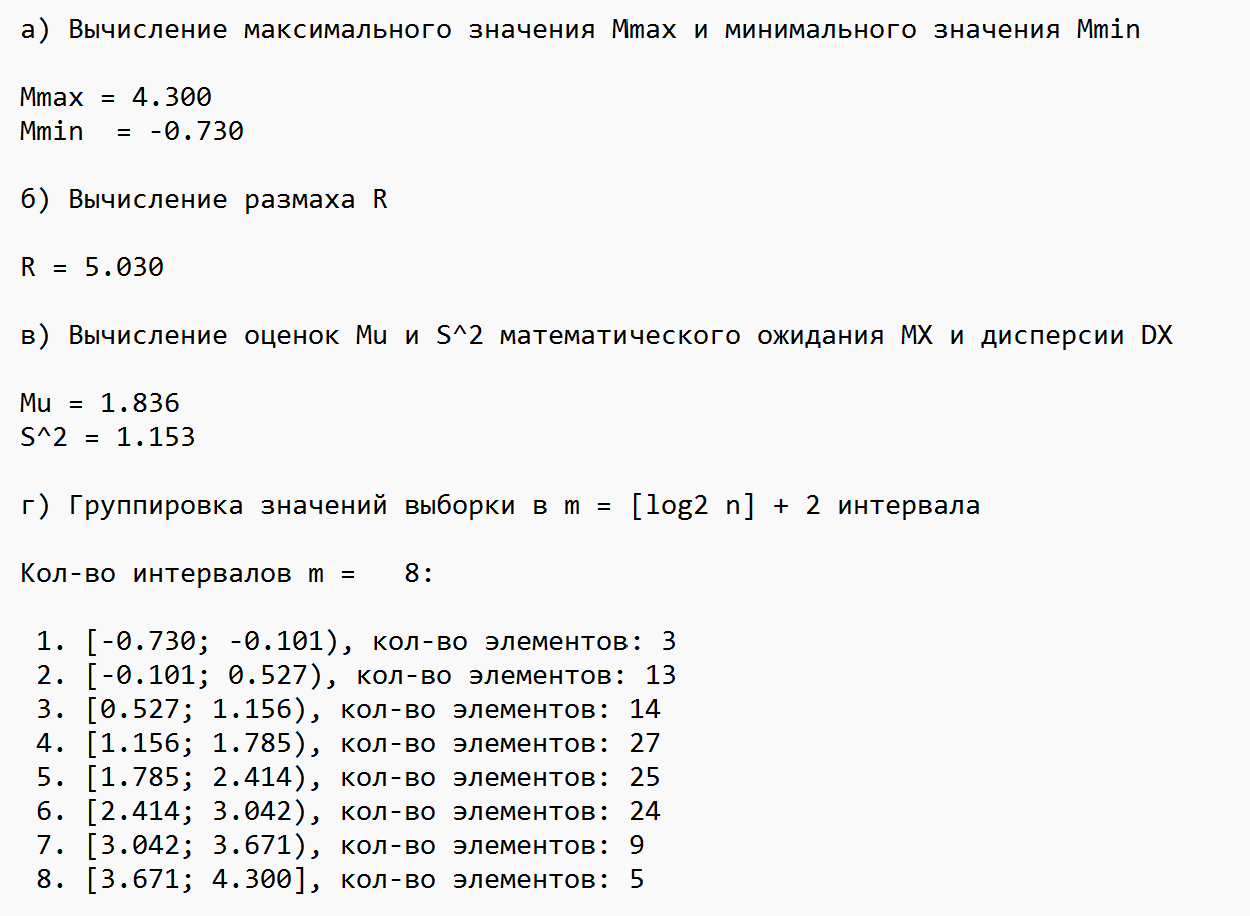
\includegraphics[scale=0.95]{images/prog_out.png}
	\caption{Результаты расчетов для выборки из 10 варианта}
	\label{fig:result}
\end{figure}

\begin{figure}[h]
	\centering
	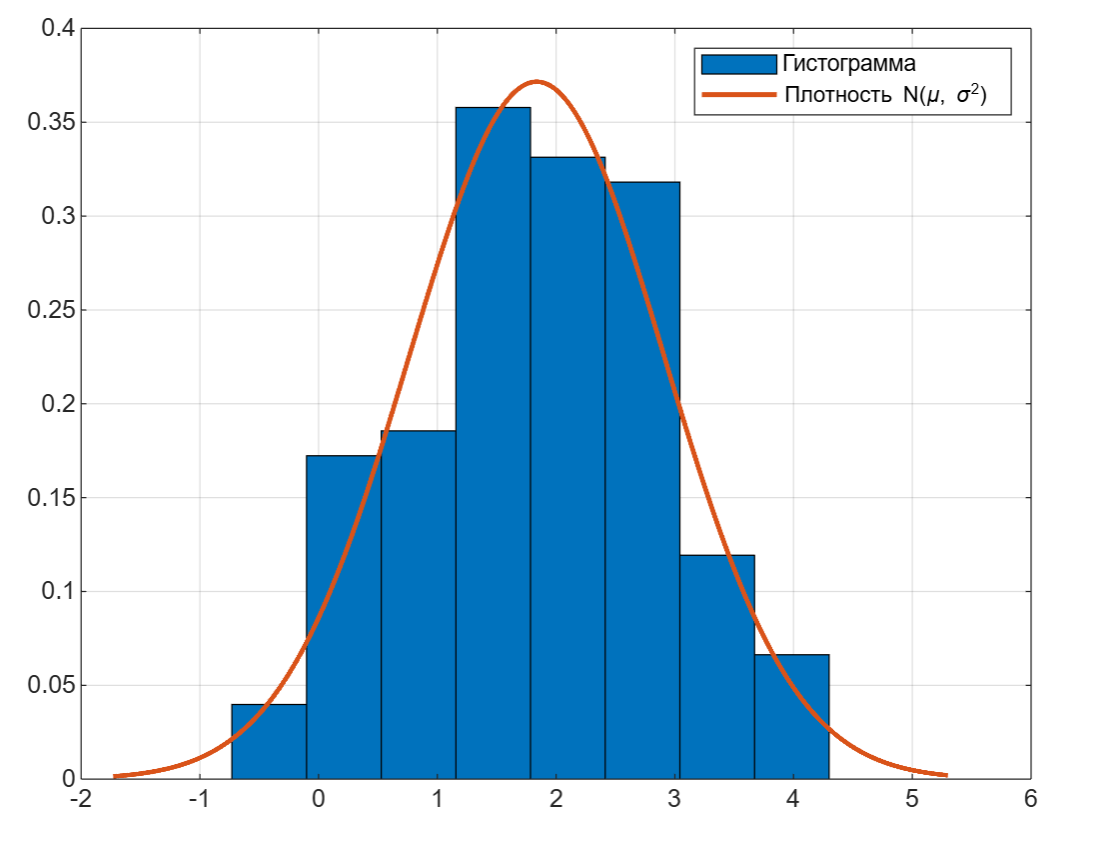
\includegraphics[scale=0.5]{images/gisto.png}
	\caption{Гистограмма и график функции плотности распределения нормальной случайной величины с выборочными математическим ожиданием и дисперсией}
	\label{fig:histo}
\end{figure}

\begin{figure}[h]
	\centering
	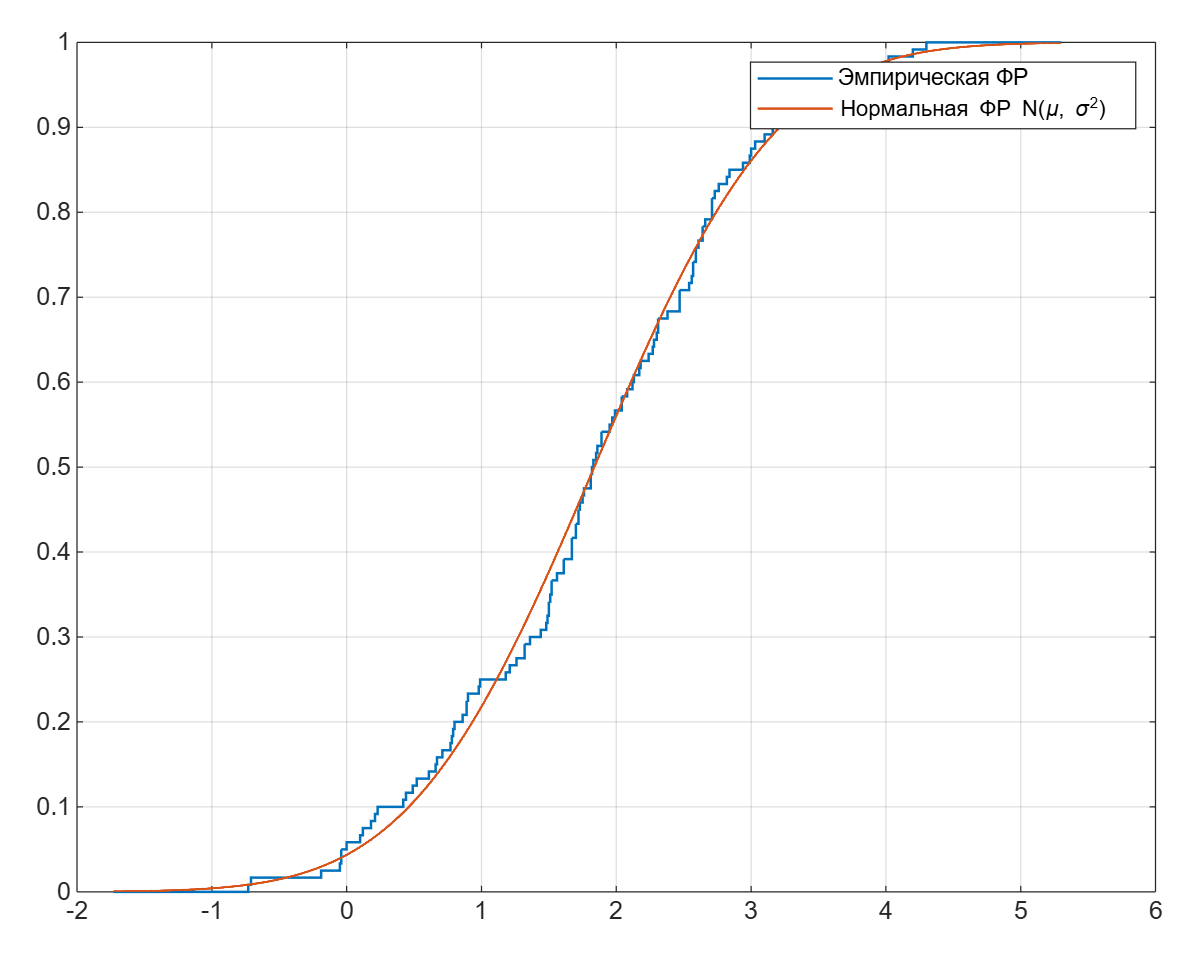
\includegraphics[scale=0.5]{images/dist_func.png}
	\caption{График эмперической функции распределения и функции распределения нормальной случайной величины с выборочными математическим ожиданием и дисперсией}
	\label{fig:emperic}
\end{figure}
